\section{Versuchsaufbau}
%skizze zum versuchsaufbau (oder foto) einf�gen,   es muss erkl�rt werden wie das ganze funktioniert und welche speziellen einstellungen verwendet wurden (z.b. welche kn�pfe an den ger�ten f�r die messung verdreht wurden)
F�r den Versuch werden zwei verscheidene Vakuumkammern verwendet. Die erste Kammer  ist eine Rutherford-Streukammer, eine schematische Skizze ist in Abb. \ref{fig:kammer} zu sehen. Die Streukammer besteht aus einer Vakuumkammer mit durchsichtigem Deckel. Ein Barometer, ein Bel�ftungsventil und ein Ventil mit Anschluss an die Vakuumpumpe sind an den Absperrhahn (3) angeschlossen. Der Halbleiterdetektor mit Kollimator (12,12.1) ist von innen an einer BNC-Buchse (2.1) montiert. Von au�en ist ein Vorverst�rker angeschlossen. die Daten werden von einem Digitalz�hler, der an einen Computer angeschlossen ist, ausgelesen (siehe Abb. \ref{fig:aufbau}). Der Deckel der Streukammer hat einen Schwenkarm (7), an dem das $^{241}$Am-Pr�parat (7.1), verschiedene Rahmen mit SpaltkKollimatoren (9) und Metallfolien (10) angebracht werden k�nnen. �ber einen Knopf (4) ist der Schwenkarm drehbar, der Winkel ist dabei �ber eine Skala (8) ablesbar. Zur Verf�gung stehen Spalte mit 1mm und 5mm Breite sowie eine Goldfolie mit 2$\mu$m und eine Aluiminiumfolie mit 7$\mu$m Dicke.

\begin{figure}[H]
	\centering
  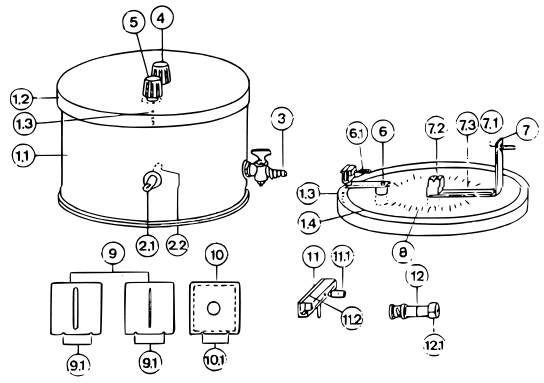
\includegraphics[scale=0.6]{streukammer.png}
	\caption{Schematischer Aufbau der Streukammer}
	\label{fig:kammer}
\end{figure}


\begin{figure}[H]
	\centering
  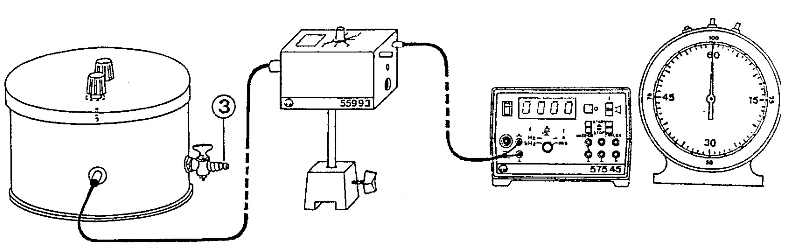
\includegraphics[scale=0.6]{aufbau.png}
	\caption{Schematischer Aufbau des Versuchsaufbaus}
	\label{fig:aufbau}
\end{figure}

Die zweite Kammer ist eine Vakuumkammer mit einer optischen Bank zum Befestigen der radioaktiven Quelle. Sie wird f�r die Bestimmung der Reichweite von $\alpha$-Strahlung und die Untersuchung der Absorbtion von verschiedenen Medien verwendet. Der Detektor ist an einen PC angeschlossen, mit dem die Messdaten aufgenommen werden.